%\documentclass[12pt,t]{beamer}
% \documentclass[t]{beamer}
\documentclass[handout]{beamer}
\usepackage{pgfpages}
\usepackage{pgffor}
\pgfpagesuselayout{4 on 1}[a4paper,landscape]

%\pagestyle{empty} % descomentar para impresión muy blanca

\usepackage[utf8]{inputenc}
\usepackage[spanish]{babel}
\decimalpoint
\usepackage{verbatim}
\usepackage{hyperref}
%\hypersetup{colorlinks=false,linkbordercolor=red,linkcolor=green,pdfborderstyle={/S/U/W 1}}
%\hypersetup{colorlinks=true,linkbordercolor=red,linkcolor=green,pdfborderstyle={/S/U/W 1}}
\hypersetup{colorlinks=true,linkcolor=blue,pdfborderstyle={/S/U/W 1}}

\usepackage{amsfonts,amssymb,amsmath,amsthm, wasysym}
\usepackage{listings}
%\usepackage[T1]{fontenc}        
\usepackage{pgf}
%\usepackage{epsdice}
\usepackage{pgfpages}
\usepackage{tikz}
\usetikzlibrary{arrows,shapes,plotmarks,backgrounds,trees,positioning}
\usetikzlibrary{decorations.pathmorphing,calc,snakes}
%\usepackage{marvosym}
%
\usetheme[hideothersubsections,left]{Marburg}
%\usetheme[hideothersubsections,left]{Madrid}
%\usetheme[hideothersubsections,left]{Dresden}
%\usetheme{Darmstadt}
\usecolortheme{sidebartab}
\useinnertheme[shadow]{rounded}

% \useoutertheme[footline=empty,subsection=true,compress]{infolines}
% \useoutertheme[footline=empty,subsection=true,compress]{miniframes}
% \usefonttheme{serif}

\setbeamertemplate{caption}[numbered]
%\setbeamertemplate{navigation symbols}{}
\addtobeamertemplate{navigation symbols}{}{%
    \usebeamerfont{footline}%
    \usebeamercolor[fg]{footline}%
    \hspace{1em}%
    \insertframenumber/\inserttotalframenumber
    
    \setbeamercolor{footline}{fg=blue}
\setbeamerfont{footline}{series=\bfseries}
}

\newcommand{\red}[1]{\textcolor{red}{#1}}
\newcommand{\green}[1]{\textcolor{green}{#1}}
\newcommand{\blue}[1]{\textcolor{blue}{#1}}
\newcommand{\gray}[1]{\textcolor{gray}{#1}}
\renewcommand{\emph}[1]{{\color{red}#1}}

%\newtheorem{theorem}



\setbeamertemplate{frametitle}
{\begin{centering}
\medskip
\color{blue}
\textbf{\insertframetitle}
\medskip
\end{centering}
}
\usecolortheme{rose}
\usecolortheme{dolphin}
\mode<presentation>


\newcommand{\CC}{\mathbb{C}}
\newcommand{\RR}{\mathbb{R}}
\newcommand{\ZZ}{\mathbb{Z}}
\newcommand{\NN}{\mathbb{N}}
\newcommand{\KK}{\mathbb{K}}
\newcommand{\MM}{\mathcal{M}}
%\newcommand{\dbinom}{\displaystyle\binom}

\newcommand{\limn}{{\displaystyle lim_{n\to\infty}}}

%\renewcommand{\lim}{\displaystyle \mathrm{lim}}
\renewcommand{\leq}{\leqslant}
\renewcommand{\geq}{\geqslant}
\def\tendeix{{\displaystyle\mathop{\longrightarrow}_{\scriptscriptstyle
n\to\infty}}}

\newcommand{\matriu}[1]{\left(\begin{matrix} #1 \end{matrix}\right)}

% \newcommand{\qed}{\hbox{}\nobreak\hfill\vrule width 1.4mm height 1.4mm depth 0mm
%     \par \goodbreak \smallskip}
%
% %

\theoremstyle{plain}
\newtheorem{teorema}{Teorema}
%\newtheorem{prop}{Proposición}
\newtheorem{prop}{Propiedades}
\newtheorem{cor}{Corolario}
\theoremstyle{definition}
\newtheorem{ejemplo}{Ejemplo}
\newtheorem{definicion}{Definición}
\newtheorem{obs}{Observación}

\newcounter{seccions}
\newcommand{\seccio}[1]{\addtocounter{seccions}{1}
\medskip\par\noindent\textbf{\theseccions.
#1}\smallskip\par }

\newcommand{\EM}{\Omega}
\newcommand{\PP}{\mathcal{P}}

\title[\red{Matemáticas III GINF}]{}
\author[]{R. Alberich}
\date{}



\usepackage{Sweave}
\begin{document}
\Sconcordance{concordance:Distribuciones_Notables.tex:Distribuciones_Notables.Rnw:%
1 238 1 48 0 4 1 12 0 10 1 17 0 18 1 4 0 107 1 12 0 11 1 17 0 18 1 %
4 0 205 1 17 0 11 1 12 0 15 1 4 0 666 1}

\beamertemplatedotitem

\lstset{backgroundcolor=\color{green!50}}
\lstset{breaklines=true}
\lstset{basicstyle=\ttfamily}


\section{Variables Aleatorias}

\begin{frame}
\vfill
\begin{center}
\gray{\LARGE Distribuciones notables}
\end{center}
\vfill
\end{frame}
\section{Distribuciones notables}

\begin{frame}
\frametitle{Introducción}
%\chapter{Distribuciones notables}
\begin{itemize}
\item En este tema estudiaremos diversos tipos de experimentos que son muy frecuentes y algunas de las variables aleatorias asociadas a ellos. 

\item Estas variables reciben distintos nombres
que aplicaremos sin distinción al tipo de población del experimento a la variable o a su
función de probabilidad, densidad o distribución.
\item Empezaremos con las variables aleatorias discretas que se presentan con frecuencia ya que están
relacionadas con situaciones muy comunes como el número de caras en varios lanzamiento de
una moneda, el número de veces que una maquina funciona hasta que se estropea, el numero de
clientes en una cola,\ldots
\end{itemize}

\end{frame}

\section{Algunas variables aleatorias discretas}
\subsection{Distribución Bernoulli}
\begin{frame}
\frametitle{Distribución Bernoulli}
\begin{itemize}
\item Consideremos un experimento con dos resultados posibles éxito (E) y
fracaso (F). El espacio de sucesos será.
\item Supongammos  que  $P(E)=p$ y entonces $P(F)=1-p=q$ con $0<p<1$.
\item Consideremos la  aplicación 
$$X:\Omega=\{E,F\}\to \RR$$
definida por
$$X(E)=1\mbox{, }X(F)=0$$
\item Su  función de probabilidad es
$$
P_{X}(x)=
\left\{
\begin{array}{ll} q & \mbox{si } x=0\\
p & \mbox{si } x=1\\
0 & \mbox{en cualquier otro caso}
\end{array}
\right.
$$
\end{itemize}
\end{frame}


\begin{frame}[fragile]
\begin{itemize}
\item Bajo estas condiciones diremos que $X$ sigue una distribución de
probabilidad  Bernoulli de parámetro $p$ y lo denotaremos por
$$X\equiv Ber(p)\mbox{ o también } X\equiv B(1,p).$$
\item A los experimentos de este tipo (éxito/fracaso)
    se les denomina experimentos Bernoulli.
\end{itemize}
\end{frame}
% 
% \begin{frame}
% \subsubsection{Resumen v.a con distribución Bernoulli, $Ber(p)$}
% 
% 
% \begin{tabular}{|c|c|c|c|c|}
% \hline \begin{tabular}{c} Valores\\ admisibles.\end{tabular} & $P_X(x)=P(X=x)=$ &
% $F_X(x)=P(X\leq X)=$ &
%  $E(X)$ & $Var(X)$\\\hline & & & &\\
%  $D_X=\{0,1\}$ & $\left\{\begin{array}{ll} q & \mbox{si } x=0\\
%     p & \mbox{si } x=1\\
%     0 & \mbox{en otro caso}\end{array}\right.$  &
% $\left\{\begin{array}{ll} 0 & \mbox{ si } x<0\\
%     q & \mbox{ si } 0\leq x<1\\
%     1 & \mbox{ si } 1\leq x \end{array}\right.$ & $p$ & $p q$ \\& & & &\\ \hline
% \end{tabular}
% \end{frame}
\subsubsection{Resumen v.a con distribución Bernoulli, $Ber(p)$}

\begin{frame}[fragile]
\frametitle{Resumen v.a con distribución Bernoulli, $Ber(p)$}
\begin{table}
\centering
\begin{tabular}{|rl|}
\hline 
\textbf{Bernoulli} & $Ber(p)$\\
\hline \hline 
$D_X=$ &  $\{0,1\}$ \\\hline 
$P_X(x)=P(X=x)=$ &  $\left\{\begin{array}{ll} q & \mbox{si } x=0\\
    p & \mbox{si } x=1\\
    0 & \mbox{en otro caso}\end{array}\right.$   \\ \hline 
$F_X(x)=P(X\leq X)=$ & $\left\{\begin{array}{ll} 0 & \mbox{ si } x<0\\
    q & \mbox{ si } 0\leq x<1\\
    1 & \mbox{ si } 1\leq x \end{array}\right.$ \\\hline 
$E(X)=$ &  $p$\\
$Var(X)=$ & $p\cdot q$\\
\hline
\end{tabular}
\end{table}
\end{frame}

\begin{frame}[fragile]

Veamos los cálculos básicos $Ber(p=0.25)$

\begin{Schunk}
\begin{Sinput}
> pbinom(0,size=1,prob=0.25)
\end{Sinput}
\begin{Soutput}
[1] 0.75
\end{Soutput}
\begin{Sinput}
> pbinom(1,size=1,prob=0.25)
\end{Sinput}
\begin{Soutput}
[1] 1
\end{Soutput}
\end{Schunk}

\end{frame}

\begin{frame}[fragile]

\begin{Schunk}
\begin{Sinput}
> dbinom(0,size=1,prob=0.25)
\end{Sinput}
\begin{Soutput}
[1] 0.75
\end{Soutput}
\begin{Sinput}
> dbinom(1,size=1,prob=0.25)
\end{Sinput}
\begin{Soutput}
[1] 0.25
\end{Soutput}
\begin{Sinput}
> rbinom(n=20,size = 1,prob=0.25)
\end{Sinput}
\begin{Soutput}
 [1] 1 0 0 0 1 0 0 0 0 1 0 0 1 0 0 1 0 0 0 0
\end{Soutput}
\end{Schunk}

\end{frame}


%\end{document}

\begin{frame}[fragile]

El siguiente código dibuja las función de probabilidad y la de distribución de una  $Ber(0.25)$

\begin{Schunk}
\begin{Sinput}
> plot(x=c(0,1),y=dbinom(c(0,1),size=1,prob=0.25),
+     ylim=c(0,1),xlim=c(-1,2),xlab="x",
+     main="Función de probabilidad\n Ber(p=0.25)")
> curve(pbinom(x,size=1,prob=0.25),
+     xlim=c(-1,2),col="blue",
+     main="Función de distribución\n Ber(p=0.25)")
\end{Sinput}
\end{Schunk}

\end{frame}


\begin{frame}[fragile]


\end{frame}


\begin{frame}[fragile]


\end{frame}

 \subsection{Distribución Binomial}
\begin{frame}

\frametitle{Distribución Binomial}

Si repetimos $n$ veces de forma independiente un experimento Bernoulli de parámetro $p$.

El espacio muestral $\Omega$ estará formado por cadenas de $E$'s y $F$'s de longitud $n$
Consideremos la v.a.

$$X(\overbrace{EFFF\ldots EEF}^{n})=\mbox{número de éxitos en la cadena}.$$

Entonces

 $$P_{X}(x)=\left\{
 \begin{array}{ll}
 \left(\begin{array}{ll} n\\
    x\end{array}\right) p^x (1-p)^{n-x} &\mbox{ si } x=0,1,\ldots,n\\
    0  & \mbox{ en otro caso}
  \end{array}\right..$$

\end{frame}

\begin{frame}

    En las anteriores circustancias diremos que la v.a. sigue una \emph{ley de probabilidad binomial con parámetros $n$ y $p$} y lo denotaremos así 
    
    $$X\equiv B(n,p).$$ 
    
    Obviamente se tiene que una bernoulli es una binomial con $n=1$
    $$B(1,p)=Ber(p).$$
\end{frame}


\begin{frame}
\frametitle{Observaciones sobre la distribución binomial}
\begin{itemize}
\item La probabilidad de fracaso la denotaremos con  $q=1-p$, sinb ningún aviso adicional.
\item Su función de distribución no tienen una formula general, por ello esta tabulada.
\item En el material de la asignatura disponéis de unas tablas de esta distribución
para distintos valores de $n$ y $p$. 
\item Cualquier paquete estadístico, hoja de cálculo,\ldots dispone de
funciones para el cálculo de estas probabilidades, así que el uso de las tablas queda \emph{totalmente anticuado}. 
\end{itemize}
\end{frame}

\begin{frame}

\frametitle{Resumen v.a con distribución binomial $B(n,p)$}
\scriptsize
\begin{table}
\centering
\begin{tabular}{|rl|}
\hline 
\textbf{Binomial} & $B(n,p)$\\
\hline \hline 
$D_X=$&  $\{0,1,\ldots n\}$ \\\hline 
$P_X(x)=P(X=x)=$ & 
$\left\{
\begin{array}{ll}
{n\choose x}\cdot  p^x\cdot  (1-p)^{n-x} & \mbox{ si } x=0,1,\ldots,n\\
     0  & \mbox{ en otro caso.}
\end{array}
\right.$
\\ \hline 
$F_X(x)=P(X\leq X)=$ & Tabulada \\\hline 
$E(X)=$ &  $n\cdot p$\\
$Var(X)=$ & $n\cdot p \cdot (1-p)$\\
\hline
\end{tabular}
\end{table}
\normalsize
\end{frame}

\begin{frame}[fragile]
\frametitle{Cálculos con R}
Veamos los cálculos básicos $B(n=10,p=0.25)$

\begin{Schunk}
\begin{Sinput}
> pbinom(0,size=10,prob=0.25)
\end{Sinput}
\begin{Soutput}
[1] 0.05631351
\end{Soutput}
\begin{Sinput}
> pbinom(1,size=10,prob=0.25)
\end{Sinput}
\begin{Soutput}
[1] 0.2440252
\end{Soutput}
\end{Schunk}

\end{frame}

\begin{frame}[fragile]
Funciones de R para la binomial 

\begin{Schunk}
\begin{Sinput}
> dbinom(0,size=10,prob=0.25)
\end{Sinput}
\begin{Soutput}
[1] 0.05631351
\end{Soutput}
\begin{Sinput}
> dbinom(1,size=10,prob=0.25)
\end{Sinput}
\begin{Soutput}
[1] 0.1877117
\end{Soutput}
\begin{Sinput}
> rbinom(n=20,size = 10,prob=0.25)
\end{Sinput}
\begin{Soutput}
 [1] 3 2 3 4 2 2 1 3 2 4 2 4 4 1 2 3 3 3 3 2
\end{Soutput}
\end{Schunk}

\end{frame}


%\end{document}

\begin{frame}[fragile]

El siguiente código dibuja las función de probabilidad y la de distribución de una  $B(n=10,p=0.25)$

\begin{Schunk}
\begin{Sinput}
> plot(x=c(0,10),y=dbinom(c(0:10),size=10,prob=0.25),
+   ylim=c(0,1),xlim=c(-1,11),xlab="x",
+   main="Función de probabilidad\n B(n=10,p=0.25)")
> curve(pbinom(x,size=10,prob=0.25),
+   xlim=c(-1,10),col="blue",
+   main="Función de distribución\n B(n=10,p=0.25)")
\end{Sinput}
\end{Schunk}

\end{frame}


\begin{frame}[fragile]


\end{frame}


\begin{frame}[fragile]


\end{frame}





\subsection{Distribución Geométrica}

\begin{frame}
\frametitle{Distribución Geométrica}

\begin{itemize}
\item Repetitamos un experimento Bernoulli, de parámetro p, de forma independiente hasta obtener el primer éxito.
\item Sea $X$ la v.a. que cuenta el número de fracasos antes del primer éxito. Por ejemplo  que  hayamos tenido  $x$ fracasos  será una cadena de $x$ fracasos culminada con un éxito. Más concretamente 

$$P(\overbrace{FFF\ldots F}^{x}E)=P(F)^{x}\cdot P(E)=(1-p)^{x}\cdot p=q^{x}\cdot p.$$
\end{itemize}
\end{frame}

\begin{frame}
Su función de probabilidad es 

$$P_X(x)=P(X=x)=\left\{\begin{array}{ll}
 (1-p)^{x} p & \mbox{ si } x=0,1,2,\ldots\\
 0 &\mbox{ en otro caso}
    \end{array}\right..$$
\begin{itemize}
\item   Una v.a. de este tipo diremos que sigue una
    distribución geométrica de parámetro $p$..
\item La  denotaremos por $Ge(p)$. 
\item Su dominio es  $D_X=\{0,1,2,\ldots\}$.
\end{itemize}
\end{frame}

\begin{frame}
\subsubsection{Propiedad de la carencia de memoria}
%\frametitle{ Propiedad de la carencia de memoria}
\begin{prop}[Propiedad de la carencia de memoria]
Sea $X$ una v.a. discreta con dominio $D_X=\{0,1,2,\ldots\}$.

Entonces $X$ sigue una ley $Ge(p)$ si y sólo si  
$$P(X\geq k+j/X> j)=P(X\geq k)$$
para todo $k,j=1,2,3\ldots$ y $P(X=1)=p$.
\end{prop}
\end{frame}

\begin{frame}

\begin{itemize}
\item  La igualdad $P(X\geq k+j/X> j)=P(X\geq k)$   significa que aunque ya llevemos más de $j$ fracasos la probabilidad de que necesitemos al menos $k$ intentos más no disminuye es la misma  que si empezáramos de nuevo el experimento. 
\item A este efecto se le suele referenciar con la frase   \emph{el experimento carece de memoria} o es un \emph{experimento sin memoria}.
\end{itemize}
\end{frame}

\begin{frame}

\subsubsection{La variable geométrica que cuenta el número de intentos}
\frametitle{La variable geométrica que cuenta el número de intentos  para obtener el
primer éxito.}

\begin{itemize}
\item Supongamos que sólo estamos interesados en el número de intentos para obtener el
primer éxito. 
\item Si definimos $Y$= número de  intentos para obtener el  primer éxito. Entonces $Y=X+1$  donde $X\equiv Ge(p)$.
\item Su dominio es
valores en $\{1,2,\ldots\}$ 
\item $E(Y)=E(X+1)=E(X)+1=\frac{1-p}{p}+1=\frac{1}{p}$.
\item $Var(Y)=Var(X+1)=Var(X)=\frac{1-p}{p^2}$.

\end{itemize}
\end{frame}


\subsubsection{Resumenes de las variables con  distribución geométrica $Ge(p)$}
\begin{frame}

\frametitle{Resumen v.a con distribución geométrica $Ge(p)$ empezando en 0}
\scriptsize
\setlength{\tabcolsep}{1pt}
\begin{table}
\centering
\begin{tabular}{|rl|}
\hline 
\multicolumn{2}{|c|}{$Y=$ número de fracasos  para conseguir el primer éxito}\\ 
\hline
\hline
\textbf{Geométrica} &  que empieza en 0\\
\hline \hline 
$D_X=$&  $\{0,1,\ldots n\}$ \\\hline 
$P_X(x)=P(X=x)=$ & 
$\left\{
\begin{array}{ll}
  (1-p)^{x}\cdot p & \mbox{ si } x=0,1,\ldots,n\\
     0  & \mbox{ en otro caso.}
     \end{array}\right.$
\\ \hline 
$F_X(x)=P(X\leq X)=$ & $\left\{\begin{array}{ll} 0 & \mbox{ si } x<0\\
  1- (1-p)^{k+1} & \mbox{ si } \left\{ \begin{array}{l}k\leq x< k+1\\\mbox{para } k=1,2,\ldots\end{array}
    \right.\end{array}\right.$ \\\hline 
$E(X)=$ &  $\frac{1-p}{p}$ \\
$Var(X)=$ & $\frac{q}{p^2}$\\
\hline
\end{tabular}
\end{table}
\normalsize

\end{frame}

% 
% \begin{frame}
% \scriptsize{
% \begin{tabular}{|c|c|c|c|c|}
%  \hline
% \multicolumn{5}{|c|}{$Y=$ número de fracasos  para conseguir el primer éxito.}\\
%  \hline \begin{tabular}{c} Valores\\ admisibles.\end{tabular} &
% $P_Y(y)=P(Y=y)=$ & $F_Y(y)=P(Y\leq y)=$&
%  $E(X)$ & $Var(X)$\\\hline & & & &\\
%   $\begin{array}{l}D_X=\\\{0,1,\ldots\}\end{array}$  & $\left\{\begin{array}{ll}
%  q^k p & \mbox{ si } k=0,1,2,\ldots\\
%  0 &\mbox{ en otro caso}
%     \end{array}\right.$  &
% $\left\{\begin{array}{ll} 0 & \mbox{si } y<0\\
%  1- q^{k+1} & \mbox{si }
%  \left\{
%  \begin{array}{l}
%  k\leq y< k+1\\
%   \mbox{para } k=0,1,2,\ldots
%  \end{array}\right.
%     \end{array}\right..$  & $\frac{1}{p}$ & $\frac{1-p}{p^2}$ \\& & & &\\ \hline
% \end{tabular}
% }
% \normalsize
% \setlength{\tabcolsep}{6pt}
% \end{frame}
% 





\begin{frame}
\subsubsection{Resumen v.a con distribución geométrica $Ge(p)$ comenzando en $1$.}

\frametitle{Resumen v.a con distribución geométrica $Ge(p)$ comenzando  en $1$}
\setlength{\tabcolsep}{1pt}
\begin{table}
\centering
\begin{tabular}{|rl|}
\hline 
\multicolumn{2}{|c|}{$X=$ número de intentos  para obtener el primer éxito}\\ 
\hline
\hline
\textbf{Geométrica} & $Ge(p)$, $q=1-p$.\\
\hline \hline 
$D_X=$&  $\{1,\ldots n\}$ \\\hline 
$P_X(x)=P(X=x)=$ & 
$\left\{
\begin{array}{ll}
  (1-p)^{x-1}\cdot p & \mbox{ si } x=1,\ldots,n\\
     0  & \mbox{ en otro caso.}
     \end{array}\right.$
\\ \hline 
$F_X(x)=P(X\leq X)=$ & $\left\{\begin{array}{ll} 0 & \mbox{ si } x<1\\
  1- q^{k} & \mbox{ si } \left\{ \begin{array}{l}k\leq x< k+1\\\mbox{para } k=1,2,\ldots\end{array}
    \right.\end{array}\right.$ \\\hline 
$E(X)=$ &  $\frac{1}{p}$ \\
$Var(X)=$ & $\frac{1-p}{p^2}$\\
\hline
\end{tabular}
\end{table}
\setlength{\tabcolsep}{6pt}
\end{frame}

\begin{frame}[fragile]
\frametitle{Cálculos con R}
Veamos los cálculos básicos con  R para la distribución geométrica  $Ge(p=0.25)$ emnpezando en $0$

\begin{Schunk}
\begin{Sinput}
> dgeom(0,prob=0.25)
\end{Sinput}
\begin{Soutput}
[1] 0.25
\end{Soutput}
\begin{Sinput}
> pgeom(0,prob=0.25)
\end{Sinput}
\begin{Soutput}
[1] 0.25
\end{Soutput}
\begin{Sinput}
> dgeom(1,prob=0.25)
\end{Sinput}
\begin{Soutput}
[1] 0.1875
\end{Soutput}
\end{Schunk}

\end{frame}

\begin{frame}[fragile]
\frametitle{Cálculos con R}
Veamos los cálculos básicos con  R para la distribución geométrica  $Ge(p=0.25)$ empezando en $0$

\begin{Schunk}
\begin{Sinput}
> pgeom(1,prob=0.25)
\end{Sinput}
\begin{Soutput}
[1] 0.4375
\end{Soutput}
\begin{Sinput}
> rgeom(n=20,prob=0.25)
\end{Sinput}
\begin{Soutput}
 [1]  3  2  5  1  1  1  0  0  0  1  1 12  4  0  8  2  3  3  4  2
\end{Soutput}
\end{Schunk}

\end{frame}

\begin{frame}[fragile]

El siguiente código dibuja las función de probabilidad y la de distribución de una  $Ge(p=0.25)$

\begin{Schunk}
\begin{Sinput}
> plot(x=c(0,10),y=dgeom(c(0:10),size=10,prob=0.25),
+   ylim=c(0,1),xlim=c(-1,11),xlab="x",
+   main="Función de probabilidad\n Ge(p=0.25)")
> curve(pgeom(x,prob=0.25),
+   xlim=c(-1,10),col="blue",
+   main="Función de distribución\n Ge(p=0.25)")
\end{Sinput}
\end{Schunk}

\end{frame}


\begin{frame}[fragile]


\end{frame}


\begin{frame}[fragile]


\end{frame}









\subsection{Distribución binomial negativa}
\begin{frame}
\frametitle{Distribución binomial negativa}
\begin{itemize}
\item 
Repetimos el
experimento hasta obtener el r-ésimo éxito. 
\item Sea $X$ la v.a que
cuenta el número de repeticiones del experimento hasta el r-ésimo
éxito. 
\item Su función de probabilidad es

{\scriptsize
     $$P_{X}(x)=P(X=x)=\left\{\begin{array}{ll}
     {{x-1}\choose{r-1}} (q)^{x-r}p^r & \mbox{si } x=r,r+1,\ldots\\
     0 & \mbox{en otro caso}\end{array}\right.$$
}
\item
     Una v.a. con este tipo de distribución recibe el nombre de \emph{binomial negativa} y la denotaremos por $BN(p,r)$. Notemos que $BN(p,1)=Ge(p)$.
\end{itemize}
%    \textbf{Nota: }
%    Se define $\left(\begin{array}{c} -nheight

%    \\ r\end{array}\right)=\frac{(-n)(-n-1)\cdots (-n-k+1)}{k!}$
%    Entonces $(t+1)^{-n}=\sum_{k=0}^{+\infty}\left(\begin{array}{c} -n
%    \\ r\end{array}\right) t^{k}$
%    Además \left(\begin{array}{c} x-1
%    \\ r-1\end{array}\right)\left(\begin{array}{c} -n
%    \\ r\end{array}\right)
\end{frame}
\subsubsection{Resumen v.a con distribución Binomial Negativa $BN(r,p)$}

\begin{frame}[fragile]
\frametitle{Resumen v.a con distribución Binomial Negativa $BN(r,p)$}
\scriptsize
\setlength{\tabcolsep}{1pt}
\begin{table}
\centering
\begin{tabular}{|rl|}
\hline
\multicolumn{2}{|c|}{$X=$ número de intentos para conseguir el $r$-ésimo éxito}\\
\hline
\hline
\textbf{Binomial negativa}  $BN(r,p)$ & $r$ éxitos, probabilidad de éxito $p$, $q=1-p$\\
\hline \hline
$D_X=$ &  $\{r,1,\ldots\}$ 
\\\hline
$P_X(x)=P(X=x)=$ &
$\left\{
\begin{array}{cc}
\left(
\begin{array}{c}
x-1\\ r-1
\end{array}
\right)\cdot
q^{x-r}\cdot p^r & \mbox{si }  x=r,r+1,\ldots \\
0 & \mbox{en otro caso.}
\end{array}
\right.$
\\
\hline
$F_X(x)=P(X\leq X)=$ & no tiene fórmula (utilizar tablas o función de R.)\\
\hline
$E(X)=$ &  $\frac{r}{p}$\\
$Var(X)=$ & $\frac{r\cdot q}{p^2}$ \\
\hline
\end{tabular}
\end{table}

\normalsize

\end{frame}

\end{document}

\subsection{Distribución Poisson}

\begin{frame}
\frametitle{Distribución Poisson}
\begin{itemize}
\item  Diremos que una v.a. discreta $X$ con $X(\Omega)=\NN$ tiene
distribución de Poisson con parámetro $\lambda>0$, y lo denotaremos
por $Po(\lambda)$ si su función de probabilidad es:

$$P_{X}(x)=P(X=x)=
\left\{\begin{array}{ll}
\frac{\lambda^x}{x!} e^{-\lambda}& \mbox{ si } x=0,1,\ldots\\
0 & \mbox{en otro caso}\end{array}\right..$$

\item Como el desarrollo en serie  Taylor de la exponencial es $e^{\lambda}=\sum_{x=0}^{+\infty} \frac{\lambda^x}{x!}$. Es fácil comprobar que  todos los valores de la función de probabilidad suman 1.
\end{itemize}
\end{frame}


\subsubsection{La distribución Poisson como ``límite'' de una binomial.}

\begin{frame}

\frametitle{La distribución Poisson como ``límite'' de una binomial.}

\begin{itemize}
\item La distribución Poisson aparece en el conteo de determinados  eventos que se
producen en un intervalo de tiempo o en el espacio.
\item Supongamos que nuestra variable de interés es  $X$= número de
eventos en el intervalo de tiempo $(0,t]$ 
\item por ejemplo el número de
llamadas a un \textsl{call center} y que sabemos que se
cumplen las siguientes condiciones:
\end{itemize}
\end{frame}



\begin{frame}
\begin{enumerate}[a)]
\item El número promedio de eventos en el intervalo $(0,t]$ es
$\lambda>0$.
\item Es posible dividir el intervalo de tiempo en un
gran número de subintervalos (denotemos por $n$ al número de intervalos) de forma que:
\begin{enumerate}[1)]
\item La probabilidad de que se produzcan dos o más eventos en un
subintervalo es despreciable.
\item El número de ocurrencias de eventos en un intervalo  es
independiente del número de ocurrencias en otro intervalo.
\item La probabilidad de que un evento ocurra en un subintervalo
es $p=\frac{\lambda}{n}$·
\end{enumerate}
\end{enumerate}
\end{frame}

\begin{frame}
\begin{itemize}
\item Bajo estas condiciones podemos considerar que el número de eventos en
el intervalo $(0,t]$ será el número de ``éxitos'' en $n$
repeticiones independientes de un proceso Bernoulli de parámetro
$p$
\item  Entonces si $n\to\infty$ y $p\cdot n$ se mantiene igual a $\lambda$
resulta que la función de probabilidad de $X$ se puede poner como

$$f_{X}(k)=\lim_{n\to\infty}\left(\begin{array}{c} n\\ k\end{array}\right)
p^k q^{n-k}= \frac{\lambda^k}{k!} e^{-\lambda}$$
\end{itemize}
\end{frame}

\begin{frame}

\begin{prop}
Si tenemos un experimento \emph{Poisson}  con $\lambda$ igual
al promedio de eventos en una unidad de tiempo (u.t.) entonces si
$t$ es una cantidad de tiempo en u.t., la v.a.
$X_{t}$=numero de eventos en el intervalo $(0,t]$
es una $Po(\lambda\cdot t)$.
\end{prop}
\end{frame}

\begin{frame}
\frametitle{Resumen v.a con distribución  Poisson  $Po(\lambda)$}
\scriptsize
\setlength{\tabcolsep}{1pt}
\begin{table}
\centering
\begin{tabular}{|rl|}
\hline 
\multicolumn{2}{|c|}{$X$ Poisson $\lambda$.}\\ 
\hline
\hline 
$D_X=$&  $\{0,1,\ldots n\}$ \\\hline 
$P_X(x)=P(X=x)=$ & 
$\left\{
\begin{array}{ll}
  \frac{\lambda^x}{x!}\exp{-\lambda} & \mbox{ si } x=0,1,\ldots,n\\
     0  & \mbox{ en otro caso.}
     \end{array}\right.$
\\ \hline 
$F_X(x)=P(X\leq X)=$ &  Función de R o tabulada \\\hline 
$E(X)=$ &  $\lambda$ \\
$Var(X)=$ & $\lambda$\\
\hline
\end{tabular}
\end{table}
\normalsize
\end{frame}





\begin{frame}


\subsubsection{Aproximación de la distribución binomial por la Poisson:}
Bajo el punto de vista anterior y si $p$ es pequeño y $n$
suficientemente grande (existen distintos criterios por ejemplo $n>20$ ó $30$ y  $p\leq 0.1$)
podemos aproximar una $B(n,p)$ por una $Po(n\cdot p)$

\subsection{Distribución hipergeométrica: }
Es la que modeliza el número de bolas blancas extraídas de una urna
sin reposición. Sea una urna que contiene $N$ bolas de las que
$N_{1}$ son blancas y las restantes $N_{2}$ no. Obviamente
$N=N_{1}+N_{2}$. Extraemos $n$ bolas de la urna sin reemplazarlas.
Sea $X$ la v.a. que cuenta el número de bolas blancas extraídas.
Entonces
$$P_{X}(x)=\left\{
\begin{array}{ll}
\frac{{{N_{1}}\choose{x}}{{N_{2}}\choose{n-x}}}{{{N}\choose{n}}} & \mbox{ si }
\max\{0,n-N_{2}\}\leq x \leq \min\{n,N_{1}\} \mbox { con } x\in \NN\\
0  & \mbox{en otro caso}\end{array}\right.$$
\end{frame}

\begin{frame}
Una v.a. hipergeométrica con los  parámetros\footnote{En ocasiones se parametriza una v.a. hipergeométrica mediante $N=$número total de bolas, 
$n$=número de extracciones y $p=$ probabilidad de una bola blanca. Así podríamos $H(N,n,p)$ donde $p=\frac{N_1}{N}$, $N=N_1+N_2$.} anteriores la
denotaremos por $H(N_1,N_2,n)$.
\end{frame}

\begin{frame}

\subsubsection{Resumen v.a con distribución hipergeométrica  $H(N_1,N_2,n)$.}
\scriptsize
\begin{tabular}{|c|c|c|c|c|}
\hline \begin{tabular}{c} Valores\\ admisibles.\end{tabular} & $P_X(x)=P(X=x)=$ &
$\begin{array}{l}F_X(x)=\\ P(X\leq X)=\end{array}$ &
 $E(X)$ & $Var(X)$\\\hline & & & &\\
 $\begin{array}{l}D_X=\\ \{x\in\NN\mid  \max\{0,n-N_{2}\}\leq x\\
 x \leq \min\{n,N_{1}\}\}
  \end{array}$ &
   $\left\{\begin{array}{ll}
     \frac{{{N_{1}}\choose{x}}{{N_{2}}\choose{n-x}}}{{{N}\choose{n}}} & \mbox{ si }
   x\in D_X
      \\ 0  & \mbox{en otro caso}\end{array}\right.$
& \begin{tabular}{c}No tiene\\ expresión.\end{tabular} & $\frac{n N_1}{N}$ & $n
\frac{N_1}{N}\left(1-\frac{N_1}{N}\right) \frac{N-n}{N-1}$
\\& & & &\\ \hline
\end{tabular}
\normalsize

\end{frame}

\begin{frame}



   \section{Algunas variables aleatorias continuas}
Al igual que en el caso discretos veremos distintos tipos de v.a. continuas que son
utilizadas de forma muy frecuente.
\end{frame}

\begin{frame}

\subsection{Distribución uniforme en el intervalo (a,b):}

Una v.a. continua $X$ diremos que tiene una distribución uniforme sobre el intervalo real
$(a,b)$ ,$(a<b)$, si su función de densidad es $$f_X(x)=\left\{\begin{array}{ll}
\frac{1}{b-a} & \mbox{si } a<x<b\\ 0  & \mbox{en cualquier otro caso}
\end{array}
\right. $$ (como ejercicio comprobar que el área comprendida entre $f_X$ y la horizontal
vale 1.)

Entonces su función de distribución es

$$F_X(x)=\left\{\begin{array}{ll} 0  & \mbox{si } x\leq a\\
\frac{x-a}{b-a} & \mbox{si } a<x<b\\ 1  & \mbox{si } b\leq x
\end{array}
\right. $$
\end{frame}

\begin{frame}

Efectivamente:

\begin{itemize}
    \item Si $x\leq a$ entonces $F_X(x)=\int_{-\infty}^{x} f(t) dt= \int_{-\infty}^{x}
    0 dt= 1\mid_{-\infty}^{x}=1-1=0$
    \item Si $a<x<b$ entonces $F_X(x)=\int_{-\infty}^{x} f(t) dt= \int_{-\infty}^{a}
    0 dt+\int_{-\infty}^{x} \frac{1}{b-a} dt= 1\mid_{-\infty}^{x}+
    \frac{t}{b-a}\mid_{a}^{x}=(1-1) +\frac{x}{b-a}-\frac{t}{b-a}=\frac{x-a}{b-a}$
    \item  Por último si $x\geq b$ entonces $F_X(x)\int_{-\infty}^{x} f(t)
    dt=1$ (ejercicio).
\end{itemize}

Si $X$ es una v.a. uniforme en el intervalo $(a,b)$ escribiremos $X\equiv U(a,b)$.
\end{frame}

\begin{frame}

\subsubsection{Esperanza y varianza  para $X\equiv U(a,b)$}

$E(X)=\int_{-\infty}^{+\infty} x f_X(x) dx=\int_{-\infty}^{+\infty} x \frac{1}{b-a} dx =
\frac{x^2}{2(b-a)}\mid _{a}^{b}=\frac{b+a}{2}$

$E(X^2)=\int_{-\infty}^{+\infty} x^2 f_X(x) dx=\int_{-\infty}^{+\infty} x^2 \frac{1}{b-a}
dx =\frac{x^3}{3(b-a)}\mid_{a}^{b} =\frac{b^3-a^3}{3(b-a)}=\frac{b^2+ab+a^2}{3}$

$Var(X)=E(X^2)-(E(X))^2=\frac{b^2+ab+a^2}{3}-(\frac{b+a}{2})^2=\frac{(b-a)^2}{12}$
%%%%%%%%\subsubsection{Gráficas de la densidad y  distribución de una uniforme}
\end{frame}

\begin{frame}

\begin{figure}[h]
\begin{center}
\begin{tabular}{cc}       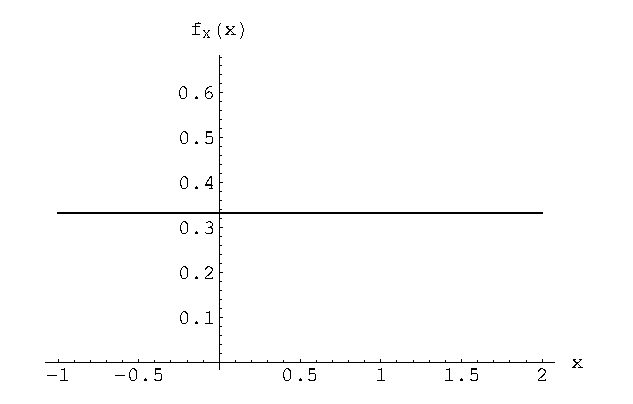
\includegraphics[scale=0.75]{densidaduniforme12}
&

       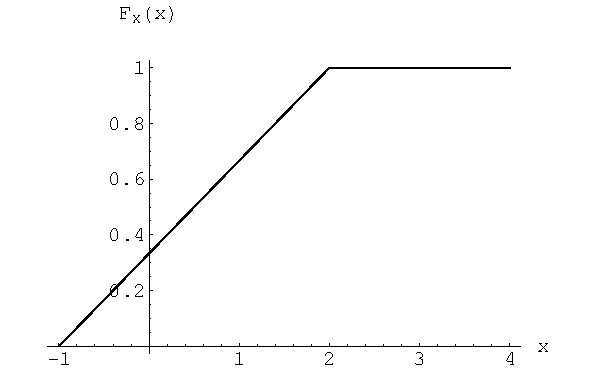
\includegraphics[scale=0.75]{distribucionuniforme12}\\ a) & b) \end{tabular}
\end{center}
       \caption{ Gráficas de la función de densidad (a)  y de la función de distribución (b) de una v.a. $U(-1,2)$.}
        \end{figure}%%%%%%%%  Sea $X$ una v.a. continua diremos que tiene distribución
%%%%%%%%          uniforme en el intervalo $(a,b)$ si su función de distribución
%%%%%%%%          es
%%%%%%%%          $$F_{X}(x)=\left\{\begin{array}{ll} 0 & \mbox{ si } x\leq a\\
%%%%%%%%          \frac{x-a}{b-a} & \mbox{ si } a\leq x\leq\\
%%%%%%%%          1 & \mbox{ si } b\leq x\end{array}\right.$$
%%%%%%%%
%%%%%%%%          $F$ es absolutamente continua y tiene por densidad:
%%%%%%%%         $$f_{X}(x)=\left\{\begin{array}{ll} \frac{1}{b-a} & \mbox{ si }
%%%%%%%%         a<x<b\\
%%%%%%%%         0 & \mbox{en el resto de casos}\end{array}\right.$$
\end{frame}

\begin{frame}



\subsubsection{Cambio lineal v.a. uniforme}


Si $X$ sigue una distribución $U(a,b)$ entonces  $Z=\frac{x-a}{b-a}$ sigue una distribución $U(0,1)$.

En general si $d$ y $e$ son dos constantes reales  $T=d\cdot X+e$ sigue una ley $U(d\cdot a +e,d\cdot b +e)$  si $d>0$, cuando $d$ sea negativo $T$ sigue una ley 
$U(d\cdot b +e,d\cdot a +e)$. Las demostración se dejan como ejercicios.

\end{frame}

\begin{frame}


\subsubsection{Resumen v.a con distribución uniforme, $U(a,b)$}

\scriptsize
\begin{tabular}{|c|c|c|c|c|}
\hline \begin{tabular}{c} Valores\\ admisibles.\end{tabular} & $f_{X}(x)$ & $F_X(x)=P(X\leq
X)=$ &
 $E(X)$ & $Var(X)$\\\hline & & & &\\
 $D_X=(a,b)$ & $\left\{\begin{array}{ll}
\frac{1}{b-a} & \mbox{si } a<x<b\\ 0  & \mbox{en cualquier otro caso}
\end{array}
\right.$  &  $\left\{\begin{array}{ll} 0 & \mbox{ si } x\leq a\\
          \frac{x-a}{b-a} & \mbox{ si } a\leq x\leq\\
          1 & \mbox{ si } b\leq x\end{array}\right.$
 & $\frac{a+b}{2}$ & $\frac{(b-a)^2}{12}$ \\& & & &\\ \hline
\end{tabular}

\normalsize

\end{frame}

\begin{frame}


         \subsection{Distribución exponencial (exponencial negativa):}
         Supongamos que tenemos un proceso Poisson con parámetro
         $\lambda$ en una unidad de tiempo.

         Sea $t$ una cantidad de tiempo en u.t. entonces $N_{t}=$ número de
         eventos en el intervalo de tiempo $(0,t]$
         es una $Po(\lambda\cdot t)$. Consideremos la v.a.
         $T=$tiempo transcurrido entre dos eventos Poisson consecutivos.

         Sea $t>0$, entonces
         $$P(T>t)=P(\mbox{Cero eventos en el
         intervalo}(0,t])
         =P(N_{t}=0)=
         \frac{(\lambda t)^0}{0!} e^{-\lambda
         t}=e^{-\lambda t}.$$

\end{frame}

\begin{frame}

         Tomando complementarios, la función de distribución de $T$ será

         $$F_{T}(t)=P(T\leq t)=\left\{\begin{array}{ll} 0 &\mbox{ si } t\leq 0\\
          1-P(T>t)=1-e^{-\lambda t}& \mbox{ si } t>0\end{array}\right.$$

         Entonces

         $$f_{T}(t)=\left\{\begin{array}{ll}
         \lambda e^{-\lambda t} & \mbox{ si }  t>0\\
         0 & \mbox{ si } t\leq 0
         \end{array}\right.$$

         La exponencial se denota por $Exp(\lambda)$
\end{frame}

\begin{frame}

\subsubsection{Propiedad de la falta de memoria}

          Sea $X$  una v.a. $Exp(\lambda)$ entonces

          $$P(X>s+t/X>s)=P(X>t)\mbox{  para todo } s,t\in \RR$$

          Toda v.a. absolutamente continua, que tome valores positivos
          y que verifique la propiedad de la falta de memoria es una v.a.
          exponencial.


\end{frame}

\begin{frame}

\subsubsection{Resumen v.a con distribución exponencial, $Exp(\lambda)$}

Sea $X\equiv Exp(\lambda).$

\scriptsize
\begin{tabular}{|c|c|c|c|c|}
\hline \begin{tabular}{c} Valores\\ admisibles.\end{tabular} & $f_{X}(x)$ & $F_X(x)=P(X\leq
X)=$ &
 $E(X)$ & $Var(X)$\\\hline & & & &\\
 $D_X=(0,+\infty)$ & $\left\{\begin{array}{ll}
         \lambda e^{-\lambda x} & \mbox{ si }  x>0\\
         0 & \mbox{ si } x\leq 0
         \end{array}\right.$ &  $F_{X}(x)=P(X\leq x)=\left\{\begin{array}{ll} 0 &\mbox{si } x\leq 0\\
          1-e^{-\lambda x}& \mbox{si } x>0\end{array}\right.
$ & $\frac{1}{\lambda}$ & $\frac{1}{\lambda^2}$ \\& & & &\\ \hline
\end{tabular}

\normalsize


\end{frame}

\begin{frame}


          \subsection{Distribución normal o Gaussiana}


          Diremos que una v.a. $X$ sigue una ley normal de parámetros
          $\mu$ y $\sigma^2$ y lo denotaremos por $N(\mu,\sigma^2)$
          si tiene por función de densidad

          $$f_{X}(x)=\frac{1}{\sqrt{2\pi}\sigma}
          e^{\frac{-(x-\mu)^2}{2\sigma^{2}}}\mbox{ para todo }x\in \RR$$

          La gráfica de esta función es la conocida campana de Gauss.

          La v.a. normal con $\mu=0$ y $\sigma=1$ recibe el nombre de
          normal estándar y se suele denotar por la letra $Z$.


%%%%%%%%          \textbf{Propiedad} Sea $X$ una v.a. $N(\mu,\sigma^2)$ y sea
%%%%%%%%          $f_{X}$ su función de densidad. Entonces:
%%%%%%%%          \vskip -1cm
%%%%%%%%          \begin{enumerate}[a)]
%%%%%%%%          \item Evidentemente $f_{X}$ verifica todas las pro\-pie\-da\-des de las
%%%%%%%%          funciones de densidad.
%%%%%%%%          \item $f_{X}(\mu-x)=f_{X}(\mu+x)$ es simétrica respecto de la recta
%%%%%%%%          $x=\mu$
%%%%%%%%          \item $f_{X}$ alcanza el máximo en $x=\mu$
%%%%%%%%         \item Si $F_{X}$ la función de distribución de $X$ entonces
%%%%%%%%         $F_{X}(\mu+x)=1-F_{X}(\mu-x)$. En par\-ti\-cu\-lar si $Z$ es una
%%%%%%%%         $N(0,1)$ entonces $F_{Z}(-x)=1-F_{Z}(x)$
%%%%%%%%         \item $Z=\frac{X-\mu}{\sigma}$ es una v.a. $N(0,1)$ y
%%%%%%%%              $X=\sigma Z+\mu$ es una $N(\mu,\sigma^{2})$ donde $Z$ es la
%%%%%%%%              normal estándar.
%%%%%%%%
%%%%%%%%          \end{enumerate}
%%%%%%%%



%%%%%%%%\section{La distribución normal o de Gauss}
%%%%%%%%
%%%%%%%% Diremos que una v.a. continua $X$ tiene
%%%%%%%%distribución normal con parámetros $\mu$ y  $\sigma^{2}$ a una variable aleatoria que tenga
%%%%%%%%por función de densidad :
%%%%%%%%$$f(x)={1\over{\sqrt{2\pi}\sigma}} {e\vphantom{A}}^{\left(-{1\over
%%%%%%%%2}{\left({x-\mu}\over{\sigma}\right)}^{2}\right)}$$
\end{frame}

\begin{frame}



\begin{figure}[h]
\begin{center}
\begin{tabular}{cc}
 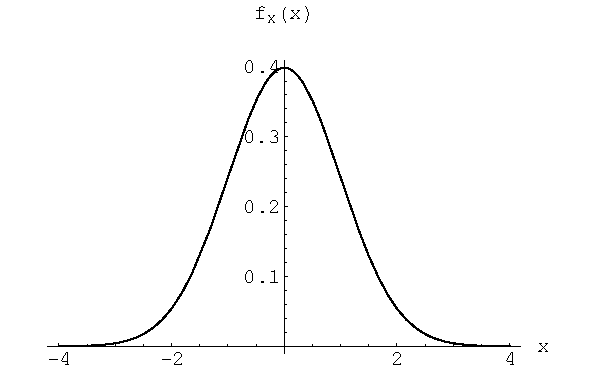
\includegraphics[scale=0.75]{densidadgaussiana}
&
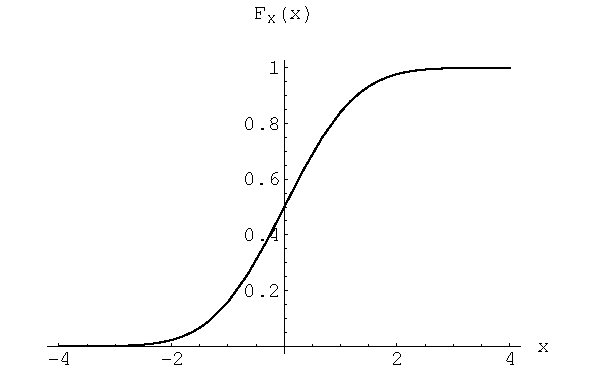
\includegraphics[scale=0.75]{distribuciongaussiana}\\ a) & b) \end{tabular}
\end{center}
       \caption{Gráficas de la función de densidad (a)  y de la  función de distribución (b) de una v.a. $N(0,1)$.}
        \end{figure}


%%%%%%%%\begin{figure}
%%%%%%%%\begin{center}
%%%%%%%%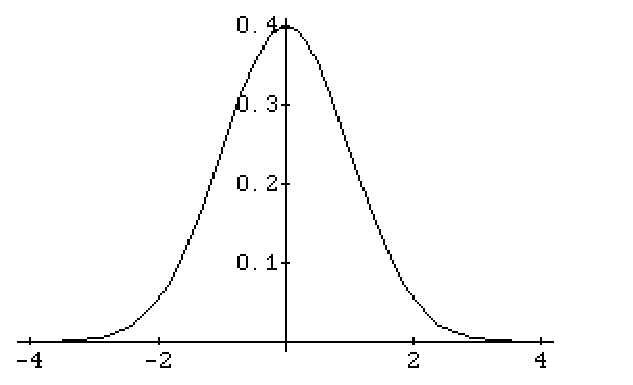
\includegraphics{normal.eps}
%%%%%%%%\end{center}
%%%%%%%%\caption{Curva de Gauss con $\mu=0$ y $\sigma=1$ }
%%%%%%%%\end{figure}

\end{frame}

\begin{frame}


Su función de distribución es, como sabemos :
$$F(x)=\int_{-\infty}^{x} {1\over{\sqrt{2\pi}\sigma}}
{e\vphantom{A}}^{-{1\over 2}{\left({t-\mu}\over{\sigma}\right)}^{2}} dt$$

Que no tiene ninguna expresión algebraica ``decente''. Es por esta razón, y  por comodidad,
que esta función está tabulada.



Cuando una variable tiene distribución normal con parámetros $\mu,\sigma$ la denotamos por
$X\equiv N(\mu,\sigma^2)$

\end{frame}

\begin{frame}

\subsubsection{Resumen v.a con distribución normal, $N(\mu,\sigma^2)$}

\scriptsize
\begin{tabular}{|c|c|c|c|c|}
\hline \begin{tabular}{c} Valores\\ admisibles.\end{tabular} & $f_{X}(x)$ & $F_X(x)=P(X\leq
X)=$ &
 $E(X)$ & $Var(X)$\\\hline & & & &\\
 $D_X=\RR$ & $=\frac{1}{\sqrt{2\pi}\sigma}
          e^{\frac{-(x-\mu)^2}{2\sigma^{2}}}\mbox{ para todo }x\in \RR$ & Tabulada la
          $N(0,1)$ & $\mu$ & $\sigma^2$ \\& & & &\\ \hline
\end{tabular}
\normalsize

\end{frame}

\begin{frame}


\subsubsection{Propiedades de la distribución normal.} La función de densidad de la
distribución normal tiene las siguientes propiedades:
\begin{enumerate}[a)]
\item $f$ es continua
\item $\int_{-\infty}^{+\infty} {1\over{\sqrt{2\pi}\sigma}} {e\vphantom{A}}^{-{1\over
2}{\left({x-\mu}\over{\sigma}\right)}^{2}} dx =1$ ( propiedad de todas las densidades).
\item $f(\mu+x)=f(\mu-x)$ y $F(x+\mu)=1-F(\mu-x)$ para todo $x\in \cal{R}$
\item $\lim\limits_{x\to+\infty}f(x)=\lim\limits_{x\to-\infty}f(x)=0$
es decir tiene asíntota horizontal a derecha e izquierda.
\item $f$ es estrictamente creciente si $x<\mu$ y decreciente si $x>\mu$.
\item Alcanza el máximo en $x=\mu$ y en este punto vale $f(\mu)=\frac{1}{\sqrt{2\pi}\sigma}$
\item Tiene dos puntos de inflexión en $x=\mu+\sigma$ y en $x=\mu-\sigma$.
\end{enumerate}
\end{frame}

\begin{frame}


\subsubsection{Transformaciones lineales de variables aleatorias normales}

\begin{prop} Sea $X\equiv N(\mu,\sigma^2)$  entonces la variable $Y=a X+b$ con
$a\not=0,b\in\cal{R}$ tiene distribución $N(a\mu+b, a^2 \sigma^2)$

En particular si  $X\equiv N(\mu,\sigma^2)$, tomando $a=\frac{1}{\sigma}$ y $b=
\frac{-\mu}{\sigma}$ la v.a. $Z={{X-\mu}\over {\sigma}}$ se distribuye $N(0,1)$.

Esta propiedad es muy importante, ya que utilizándola sólo necesitaremos tabular la
$N(0,1)$. A la función de distribución de una $Z\equiv N(0,1)$ la llamaremos $F_Z$  y a una
normal $N(0,1)$  se le denomina normal estándar. Por lo tanto si
$F_X(x)=F_Z(\frac{x-\mu}{\sigma})$.
\end{prop} 

La propiedad siguiente se desprende de las propiedades generales de una normal y nos será
muy útil en los cálculos de probabilidades de una normal.
\end{frame}

\begin{frame}

\textbf{Propiedad} Si $Z\equiv N((0,1)$ entonces $F_{Z}(x)=1-F_{Z}(-x)$.

\begin{example} Sea $Z\equiv N(0,1)$  Calcular :
\begin{enumerate}[a)]
\item Dado $\delta>0$, $P(-\delta\leq Z \leq
\delta)=F_{Z}(\delta)-F_{Z}(-\delta)=F_Z(3)-(1-F_Z(\delta))=2 F_Z(\delta)-1$
\item $P(-4\leq Z \leq 4)=F_{Z}(4)-F_{Z}(-4)=2 F_Z(4)-1$
\item $P(-2\leq Z \leq 2)=F_{Z}(2)-F_{Z}(-2)=2 F_Z(2)-1$
\item $P(Z\leq -2)=F_Z(-2)=1-F_Z(2)$
\item $P( Z \leq 2)=F_{Z}(2)$
\item $P( Z \geq 2)=1-P(Z<2)=1-F_{Z}(2)$
\item $P( Z > 2)=1-P(Z\leq 2)=1-F_{Z}(2)$
\item $P( Z = 2)=0$
\item $P( Z \geq -2)=1-P(Z< -2)=1-F_{Z}(-2)=1-(1-F_Z(2))=F_Z(2).$
\end{enumerate}
\end{example}


\end{frame}

\begin{frame}

    Resumiendo podemos utilizar las siguientes propiedades, $X\equiv N(\mu,\sigma)$
    \begin{itemize}
    \item  $Z$ es su variable tipificada, es decir,
    $Z=\frac{X-\mu}{\sigma}\equiv N(0,1)$ entonces:

    $$P(X\leq x)=P(\frac{X-\mu}{\sigma}\leq
    \frac{x-\mu}{\sigma})=F_{Z}(\frac{x-\mu}{\sigma})$$

   \item  Cuando tengamos un intervalo
    $$P(a<X<b)=P(\frac{a-\mu}{\sigma}<\frac{X-\mu}{\sigma}<\frac{b-\mu}{\sigma})=$$

    $$=P(\frac{a-\mu}{\sigma}<Z<\frac{b-\mu}{\sigma})=F_{Z}(\frac{b-\mu}{\sigma})-
    F_{Z}(\frac{a-\mu}{\sigma})$$
    \item Si $\delta>0$ $P(\mu-\delta\leq X \leq
\mu+\delta)=2 F_Z(\frac{\delta}{\sigma})-1$
\end{itemize}
\end{frame}
%\end{document}
\begin{frame}

\frametitle{Ejemplo}
Sea $X$ una normal com media $2$ y varianza $4$, entonces
\begin{enumerate}[a)]
\item  $P(1< X< 2)= P(\frac{1-2}{2}<\frac{X-2}{2}<\frac{2-2}{2})=P(\frac{-1}{2}<Z<0)=F_{Z}(0)-F_{Z}(-0.5)=\frac{1}{2}-1+F_{Z}(0.5).$
\item $P(X>3)=P(\frac{X-2}{2}>\frac{3-2}{2})=P(Z>0.5)=1-F_{Z}(0.5).$
\end{enumerate}
\end{frame}

\end{document}
